\documentclass[11pt,letterpaper]{article}
\usepackage[utf8]{inputenc}

%----- Configuración del estilo del documento------%
\usepackage{epsfig,graphicx}
\usepackage[left=2cm,right=2cm,top=1.8cm,bottom=2.3cm]{geometry}
\usepackage{fancyhdr}
\usepackage{lastpage}
\pagestyle{fancy}
\fancyhf{}

\usepackage{amsmath,amsthm,amssymb, tikz}
\usepackage{graphicx}
%%Use this package for matrices
\usepackage{array}
\usepackage{breqn}
\usepackage{multicol}
\usepackage{lipsum}
\usepackage{caption}
\usepackage{subcaption}
\usepackage{booktabs}

%%%%%%%%%%%%%%%%%%%%%%%%%%%%%%%%%%%%%%%%%%%%%%%%%%%%%%%%%%%%%%%%%%%%%%%%%%%%%%%%
\usepackage{amsmath}
\usepackage{amssymb}
\usepackage{graphicx}
\usepackage{subcaption}
\usepackage{mwe}
\usepackage{amsthm}
\usepackage{float}
\usepackage[export]{adjustbox}
\DeclareMathOperator*{\argmin}{argmin} 

%%%%%%%%%%%%%%%%%%%%%%%%%%%%%%%%%%%%%%%%%%%%%%%%%%%%%%%%%%%%%%%%%%%%%%%%%%%%%%%%

\usepackage{lipsum}



\begin{document}

%%%%%%%%%%%%%%%%%%%%%%%%%%%%%%%%%%%%%%%%%%%%%%%%%%%%%%%%%%%%%%%%%%%%%%%%%%%%%%%%

\begin{center}
    \begin{minipage}{10cm}
    	\begin{center}
    	\textbf{\large Project 4 Regression Analysis}\\[0.1cm]
        \textbf{Inesh Chakrabarti, Lawrence Liu, Nathan Wei}\\[0.1cm]
    	\end{center}
    \end{minipage}\hfill
\end{center}

\rule{17cm}{0.1mm}

%%%%%%%%%%%%%%%%%%%%%%%%%%%%%%%%%%%%%%%%%%%%%%%%%%%%%%%%%%%%%%%%%%%%%%%%%%%%%%%%

\section*{Introduction}
For the first part of this project we will do regression analysis. The dataset 
we chose to use is one of diamond characteristics. We will conduct regressions
to predict the price of a diamond given some features. 


\section*{Dataset}
Let us begin by understanding the dataset. The dataset consists of information
about 53940 round-cut diamonds with ten features: 
\begin{table}[ht]

\label{table1} 
\begin{tabular}{cl} 
\hline
\multicolumn{1}{c}{Feature} & \multicolumn{1}{c}{Description}\\
\hline 
    \texttt{carat} & weight of the diamond (0.2–5.01) \\
    \texttt{cut} & quality of the cut (Fair, Good, Very Good, Premium, Ideal) \\
    \texttt{color} & diamond colour, from J (worst) to D (best) \\
    \texttt{clarity} & a measurement of how clear the diamond is (I1 (worst),  
    SI2, SI1, VS2, VS1, VVS2, VVS1, IF (best)) \\
    \texttt{x} & length in mm (0–10.74) \\
    \texttt{y} & width in mm (0–58.9) \\
    \texttt{z} & depth in mm (0–31.8) \\
    \texttt{depth} & total depth percentage \\
    \texttt{table} & width of top of diamond relative to widest point (43-95) \\
    \texttt{price} & price in US dollars (\$326-\$18,823)
\end{tabular}
\end{table}


%%%%%%%%%%%%%%%%%%%%%%%%%%%%%%%%%%%%%%%%%%%%%%%%%%%%%%%%%%%%%%%%%%%%%%%%%%%%%%%%

\subsubsection*{Question 1.1}
\begin{figure}[H]
    \centering
   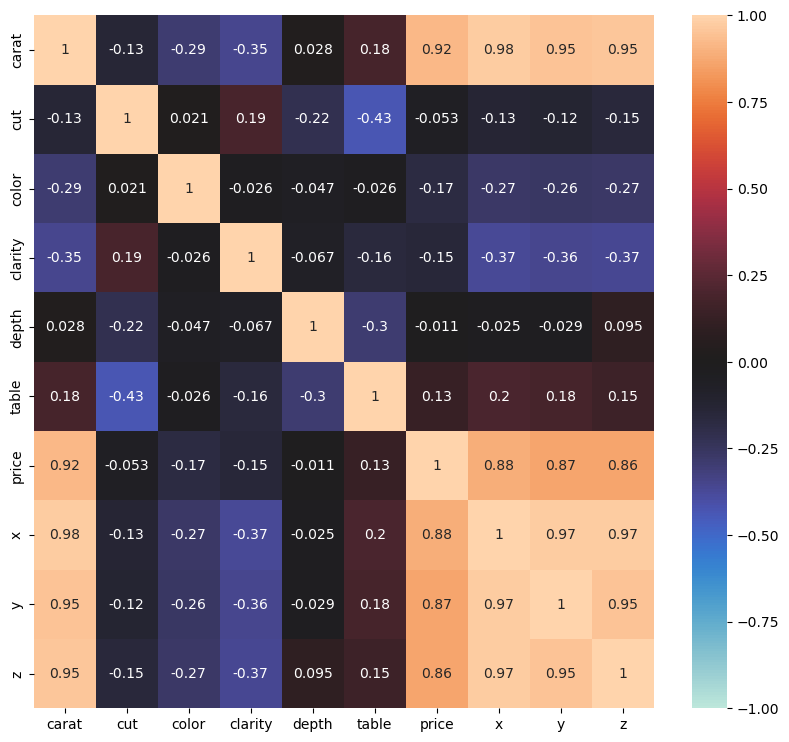
\includegraphics[width=0.5\linewidth]{../Figures/Question-1/datasetCorrHeatmap.png}
   \caption{Feature Pearson Correlation Heatmap}
   \label{fig:corr_hm}
\end{figure}

We will be using the nine features to predict the \texttt{price}. We can begin by 
computing the Pearson correlation matrix heatmap for these features in 
the dataset in Figure 1. Note that a pearson correlation coefficient $r$ is 
defined as such:
\begin{equation}
r=\dfrac{\sum_i \left(x_i-\bar{x}\right)\left(y_i-\bar{y}\right)}{\sqrt{
\sum_i\left(x_i-\bar{x}\right)^2\sum_i\left(y_i-\bar{y}\right)^2
}}
\end{equation}
We have assigned quantitative values to
the qualitative labels \texttt{cut},\texttt{color},\texttt{clarity} as ascending 
natural numbers based on ideality.

\begin{table}[H]
    \begin{subtable}[H]{0.45\textwidth}
        \centering
        \begin{tabular}{c l}
            \hline
            Feature & \multicolumn{1}{c}{Correlation}         \\
            \hline 
        \texttt{carat}   & 0.9215914337868304    \\
        \texttt{cut}     & -0.05349263851362828  \\
        \texttt{color}   & -0.1725093772499559   \\
        \texttt{clarity} & -0.14680175361025616  \\
        \texttt{depth}   & -0.010647725608533299 \\
        \texttt{table}   & 0.12713358133531918   \\
        \texttt{x}       & 0.8844357793744166    \\
        \texttt{y}       & 0.865421694764742     \\
        \texttt{z}       & 0.861250266123968    
        \end{tabular}
        \caption{Price}
        \end{subtable}
        \begin{subtable}[H]{0.45\textwidth}
            \centering
            \begin{tabular}{c l}
                \hline
                Feature & \multicolumn{1}{c}{Correlation}         \\
                \hline 
            \texttt{carat}   & 0.7694571626172851    \\
            \texttt{cut}     & 0.00542011950342582   \\
            \texttt{color}   & -0.011980043670033661 \\
            \texttt{clarity} & 0.04512538515850012   \\
            \texttt{depth}   & -0.03572374489729493  \\
            \texttt{table}   & 0.08458507638109278   \\
            \texttt{x}       & 0.7873455524189906    \\
            \texttt{y}       & 0.7717301198408058    \\
            \texttt{z}       & 0.7655421629234554   
            \end{tabular}
            \caption{Price per Carart}
        \end{subtable}
        \caption{Pearson Correlation Coefficients}
    \end{table}

The values for correlation for \texttt{price} is given in 
Table 1(a). We see that, unsurprisingly, there is a massive collection of high 
correlation squares at the bottom right. These indicate high Pearson 
correlation coefficient between \texttt{price} and \texttt{x}, \texttt{y}, 
\texttt{z}. Similarily, there is also a high correlation with \texttt{carat}.
All of these suggest that the size of the diamond itself is the most significant 
predictor as to its price. \\ 

However, unexpectadly, we had a negative perason coeffciient for the quality of 
the \texttt{cut}, \texttt{color}, and \texttt{clarity}. This was odd, so we
similarily calculated the Pearson correlation values for Price per Carat instead, 
given in Table 1(b). We observed that the coefficient for \texttt{cut} and 
\texttt{clarity} became slightly positive, while color became close to zero. 
These seemed more in line with our expectations,and confirmed that the rarity of 
high carat and high clarity in a diamond at the same time was making the 
corresponding values in Table 1(a) negative. 

\subsubsection*{Question 1.2}
\begin{table}[H]
    \begin{subtable}[H]{0.45\textwidth}
    \centering
    \begin{tabular}{c l}
        \hline
        Feature & \multicolumn{1}{c}{Skewness} \\
        \hline
        \texttt{carat} & 1.116645920812613  \\ \
        \texttt{depth} & -0.08229402630189467 \\ \
        \texttt{table} &  0.7968958486695427\\ \
        \texttt{x} & 0.3786763426463927  \\ \
       \texttt{y} & 2.4341667164885554  \\ \
        \texttt{z} & 1.5224225590685583  \\ \
    \end{tabular}
    \caption{Before Processing}
    \end{subtable}
    \begin{subtable}[H]{0.45\textwidth}
        \centering
        \begin{tabular}{c c l}
            \hline
            Feature & Method & \multicolumn{1}{c}{Skewness} \\
            \hline
            \texttt{carat} & Box Cox & 0.020450070764268666 \\ \
            \texttt{depth} & No Change & -0.08229402630189467 \\ \
            \texttt{table} &  Box Cox & 0.020450070764268666\\ \
            \texttt{x} & No Change & 0.3786763426463927  \\ \
           \texttt{y} & Box Cox & 0.020450070764268666  \\ \
            \texttt{z} & Square Root & 0.0139742634447758  \\ \
        \end{tabular}
        \caption{After Processing}
        \end{subtable}
    \caption{Skewness of Features}
\end{table}

\begin{figure}[H]
    \centering
    \begin{subfigure}[b]{0.45\textwidth}
        \centering
        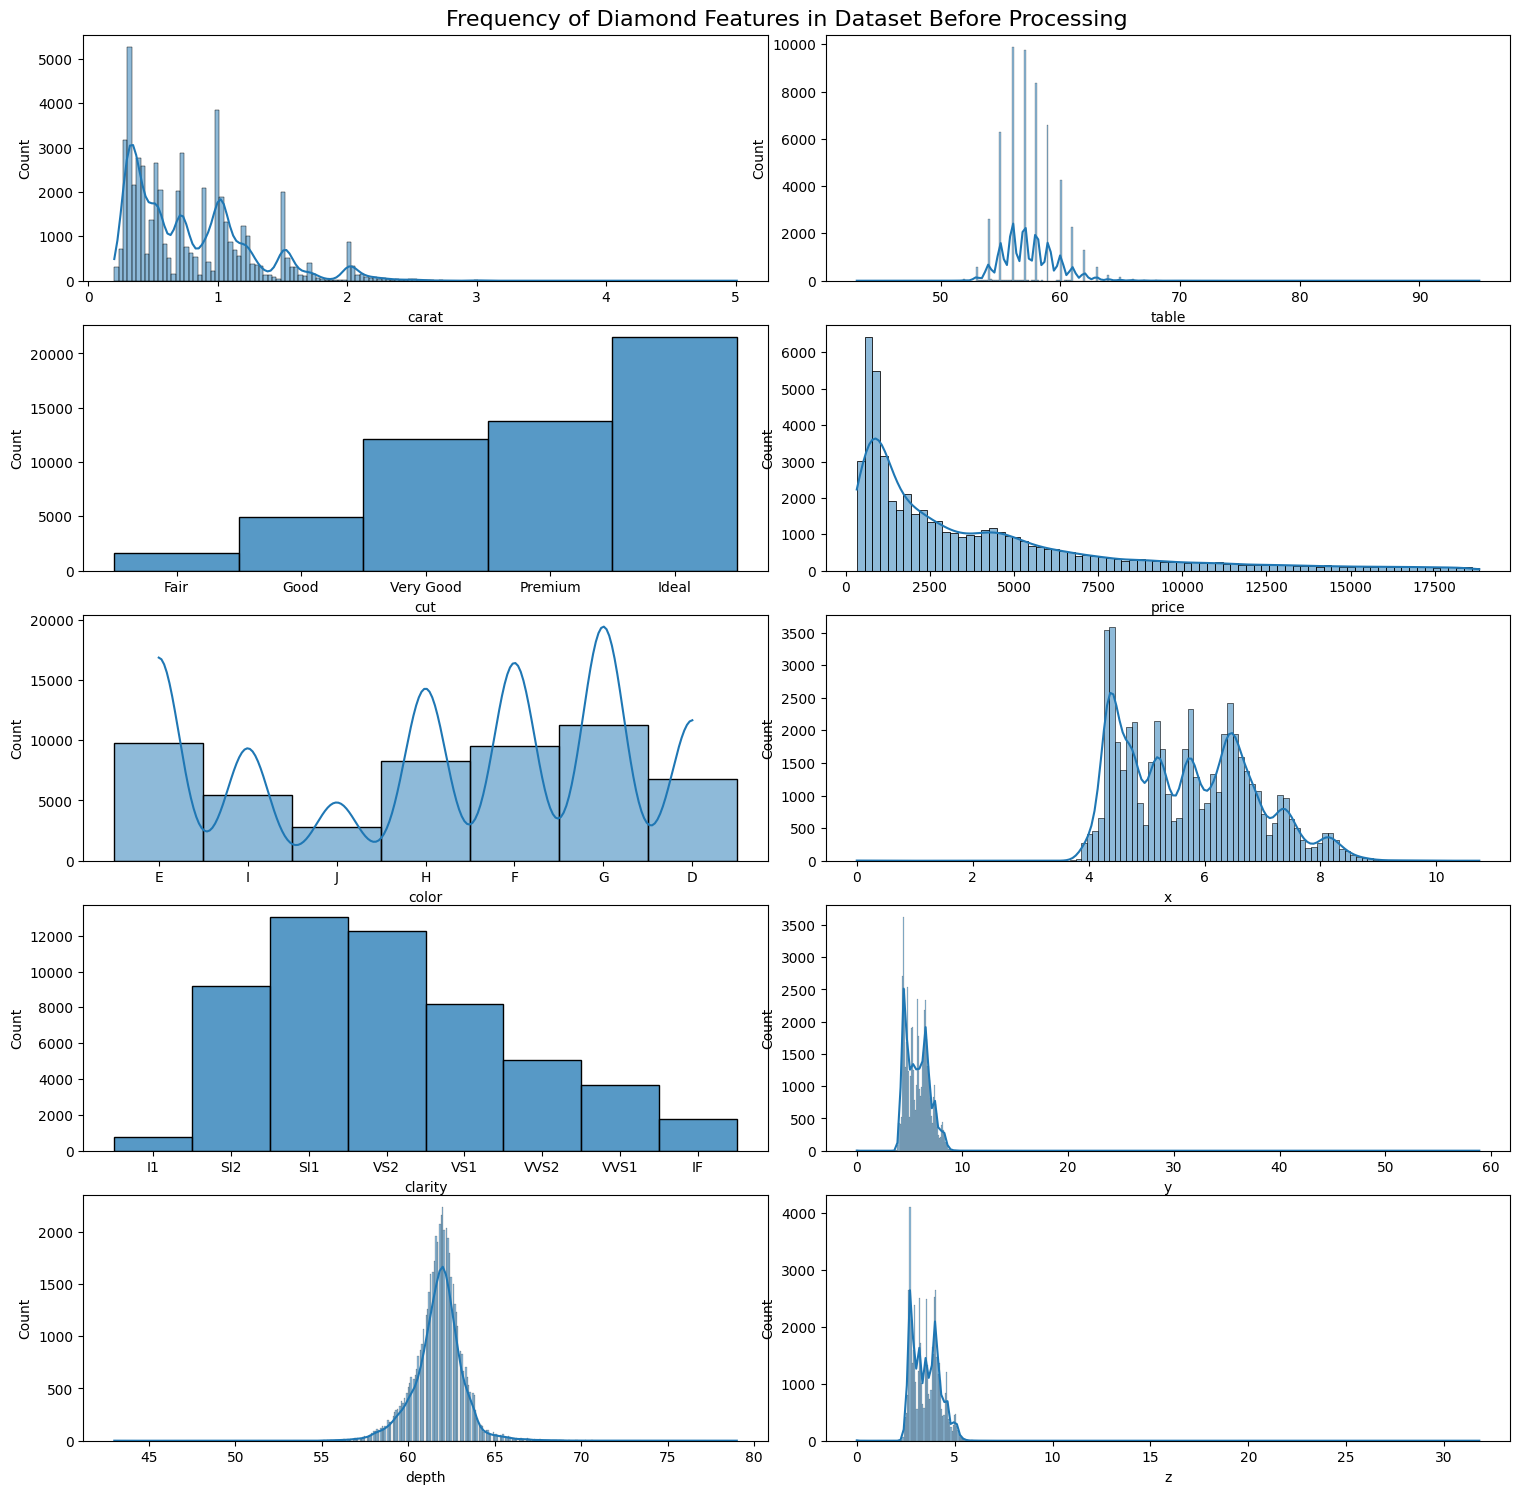
\includegraphics[width=\textwidth]{../Figures/Question-1/featureprehist.png}
        \caption{Before Processing}
        \label{fig:clarityBox}
    \end{subfigure}
    \hfill
    \begin{subfigure}[b]{0.45\textwidth}
        \centering
        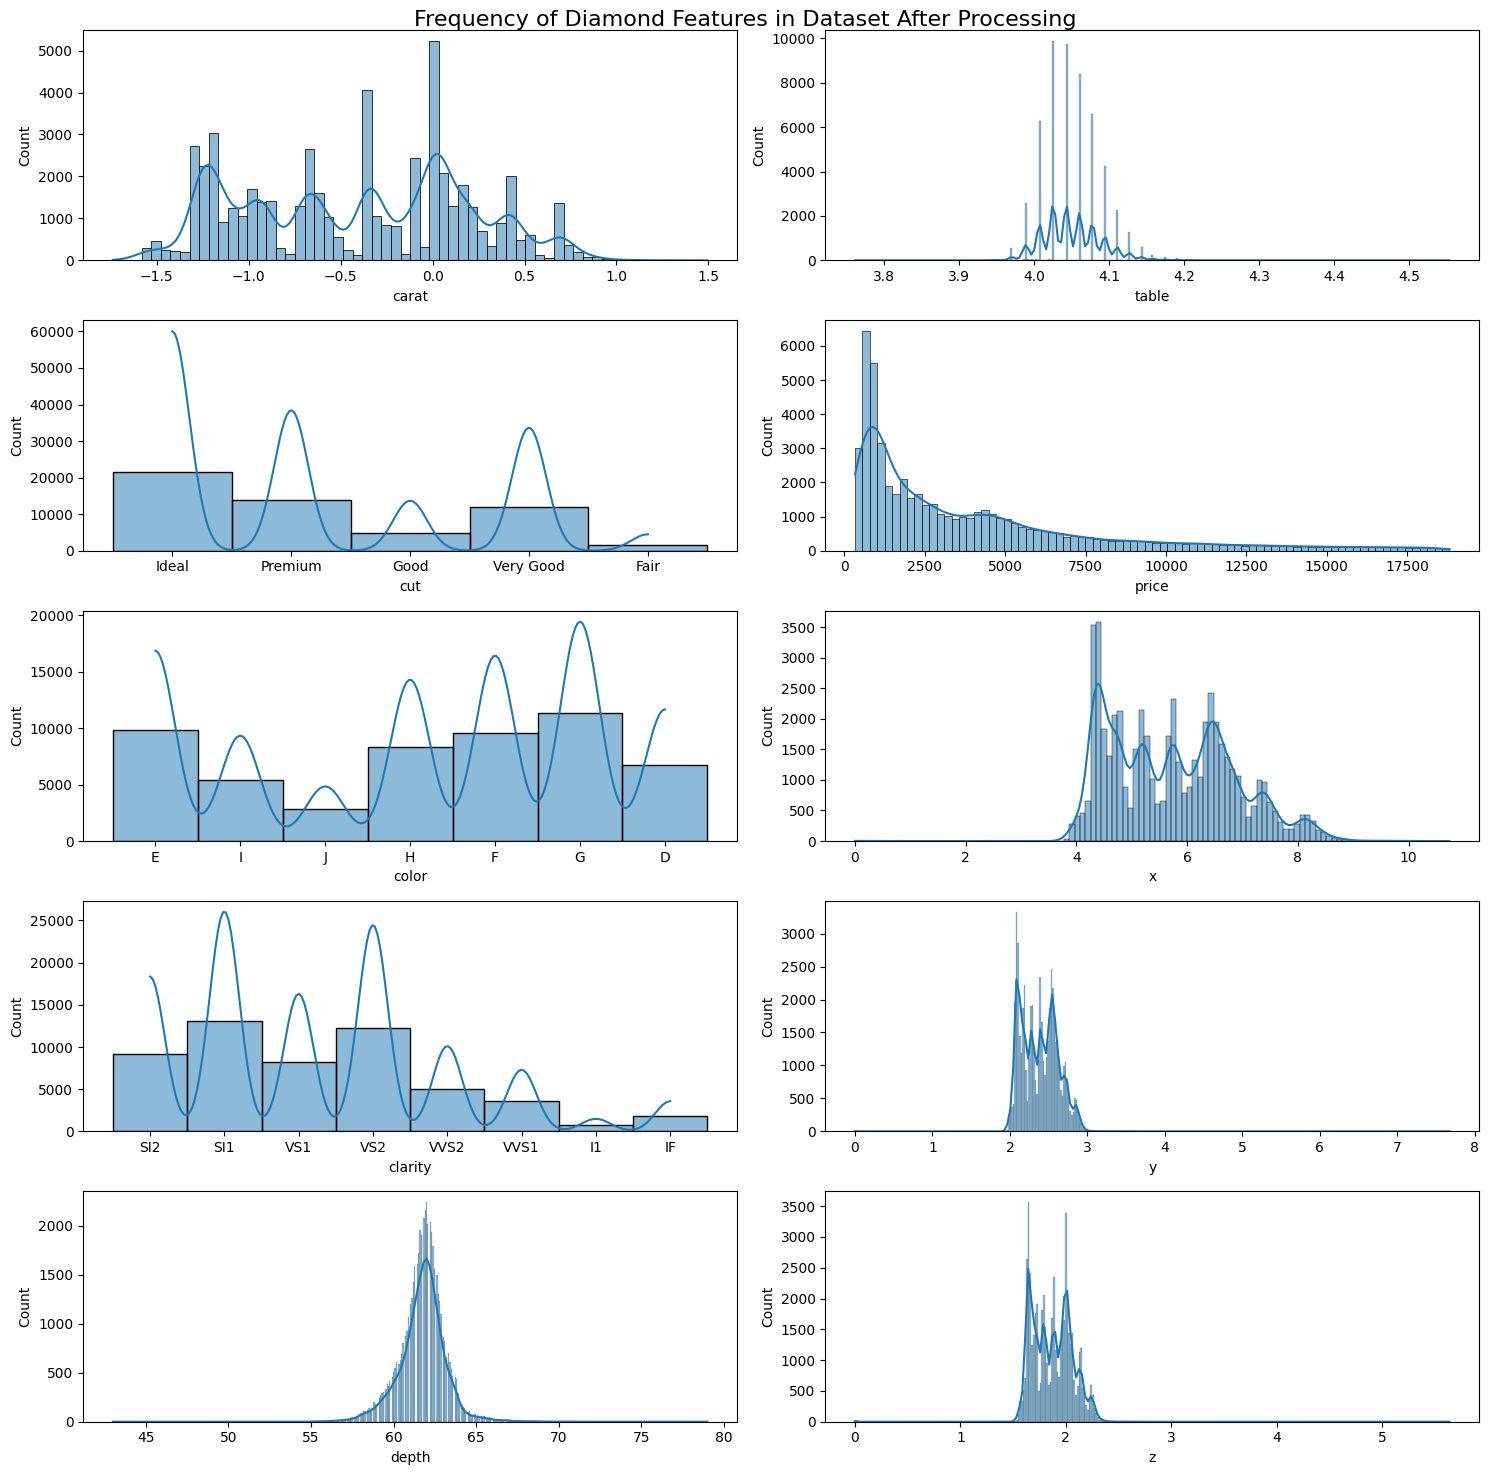
\includegraphics[width=\textwidth]{../Figures/Question-1/featureposthist.png}
        \caption{After Processing}
        \label{fig:colorBox}
    \end{subfigure}
       \caption{Histogram and KDE for Features}
       \label{fig:boxPlots}
\end{figure}

%%%%%%%%%%%%%%%%%%%%%%%%%%%%%%%%%%%%%%%%%%%%%%%%%%%%%%%%%%%%%%%%%%%%%%%%%%%%%%%%
Now, we examine the frequency distributions within each feature. We find that 
some of our numerical features are somewhat skewed—apparent from Table 2(a) and
Figure 2(a). We target a skewness less than $0.5$, as this would imply that the 
distribution is somewhat symetric. As such, we try three different methods: 
square-root, logrithm, and box-cox transformation. The first two are somewhat
self-explanatory; box-cox uses a non-zero value of $\lambda$ and conducts the
following transformation:
\begin{equation}
y_{\lambda}^{'} = \dfrac{y^{\lambda}-1}{\lambda \cdot \bar{g}_y^{\lambda-1}}
\end{equation}
where $\bar{g}_y$ is defined as the geometric mean of $y$. \\
We next try all of these methods, along with no transformatino, and take the 
minimum to try to minimize skewness in our data. The results are shown in Table 
2(b) and Figure 2(b).


\subsubsection*{Question 1.3}

\begin{figure}[H]
    \centering
    \begin{subfigure}[b]{0.3\textwidth}
        \centering
        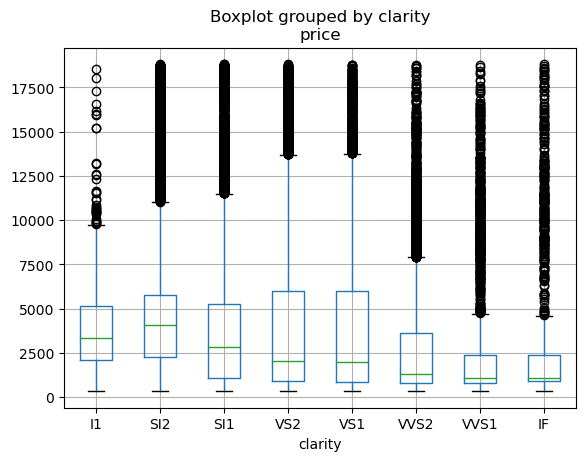
\includegraphics[width=\textwidth]{../Figures/Question-1/clarityBox.png}
        \caption{Clarity}
        \label{fig:clarityBox}
    \end{subfigure}
    \hfill
    \begin{subfigure}[b]{0.3\textwidth}
        \centering
        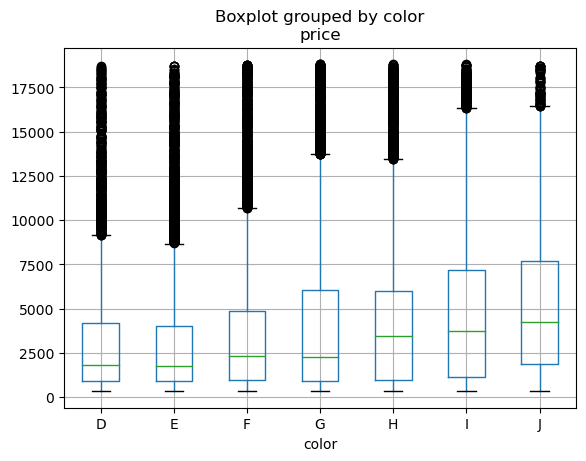
\includegraphics[width=\textwidth]{../Figures/Question-1/colorBox.png}
        \caption{Color}
        \label{fig:colorBox}
    \end{subfigure}
    \hfill
    \begin{subfigure}[b]{0.3\textwidth}
        \centering
        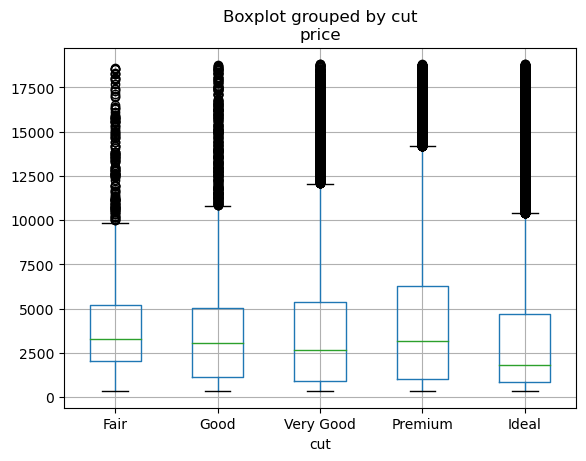
\includegraphics[width=\textwidth]{../Figures/Question-1/cutBox.png}
        \caption{Cut}
        \label{fig:cutBox}
    \end{subfigure}
       \caption{Categorical feature vs price boxplots}
       \label{fig:boxPlots}
\end{figure}

We see that idek what the fuck we see bro??

\subsubsection*{Question 2.1}
Now, before we train our regression models, we begin by splitting our data into 
training and testing sets. As such, we must now standardize the feature columns.
The function used to do this, \texttt{scaledTrainTest()}, as well as \texttt{
scaledTrainTestSplit()} can be found in \texttt{utils.py}.

\subsubsection*{Question 2.2}
Next, we begin with feature selection. We note that some of the features may not
be useful or may cause overfitting in our models as they do not carry useful 
useful information about the variable that we are trying to predict. To tell 
whether this is the case, we use two metrics: Mutual Information (MI) and F 
score.

\begin{figure}[H]
    \centering
   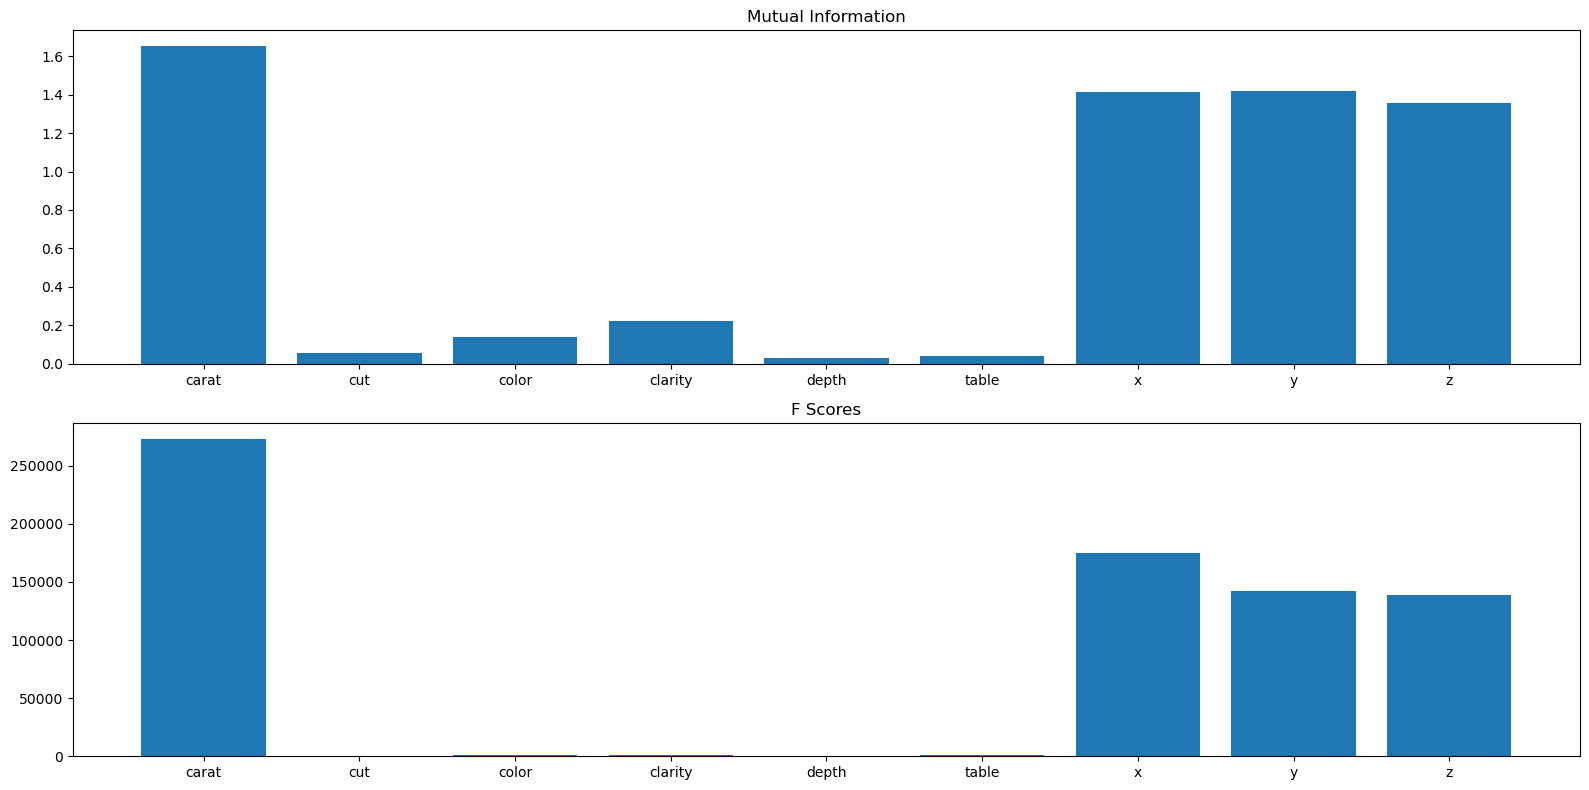
\includegraphics[width=0.8\linewidth]{../Figures/Question2/mi.png}
   \caption{Bar graph of F score and Mutual Information for features}
\end{figure}
\begin{table}[!ht]
    \centering
    \begin{tabular}{c l l}
    \hline
        Feature & Mutual Information & F Score \\ \hline
        \texttt{carat} & 1.64589286853222835 & 273144 \\ \
        \texttt{cut} &0.058351547792578895 & 139 \\ \
        \texttt{color} &0.13968295427702282 & 1465 \\ \
        \texttt{clarity} & 0.21672877051000627 & 1079 \\ \
        \texttt{depth} & 0.030486803506200033 & 5.074 \\ \
        \texttt{table} & 0.03818752327438668 & 802 \\ \
        \texttt{x} & 1.4058664238563194 & 174973 \\ \
       \texttt{y} & 1.4172107199595354 & 142130 \\ \
        \texttt{z} & 1.3569258463570115 & 138947 \\ \
    \end{tabular}
    \caption{Mutual Information and F Score Values for features}
\end{table}
It is clear by observation from Figure 3 and Table 2 that the lowest mutual 
information is present in \texttt{depth} and \texttt{table}. It is also 
important to note that the mutual information in \texttt{cut} is also very small. 
This makes sense as we saw earlier that the Pearson correlation coefficient for 
\texttt{cut} with respect to price per carat was almost zero. Similarily, the 
Pearson correlation coefficients for depth and table were very close to zero. \\ 

From this point, we will be testing the regression models without these three 
features, and with these three features and comparing the performance to 
determine the general performance.

\section*{Regression Models}
\subsubsection*{Question 3}
%%%%%%%%%%%%%%%%%%%%%%%%%%%%%%%%%%%%%%%%%%%%%%%%%%%%%%%%%%%%%%%%%%%%%%%%%%%%%%%%
For this entire section we perform 10-fold cross validation and then measure
the average RSME error for the training and validation sets. For the random 
forest model we also measure "Out-of-Bag Error" and $R^2$ score. \\
"Out-of-Bag Error" refers to 
\subsection*{Linear Regression}
\subsubsection*{Question 4.1}
We begin with a simple regression, least square linear regression. Begin by 
noting the optimization problem:
\begin{equation}
    \argmin_{\theta} \dfrac{1}{2}||\textbf{Y}-\theta^T\hat{\textbf{X}}||^2
\end{equation}
Taking the derivative with respect to $\theta$ and setting it equal to zero 
gives us 
\begin{equation}
\theta = \left(\textbf{X}^T\textbf{X}\right)^{-1}\textbf{X}^T\textbf{Y}
\end{equation}
Now, we can add regularization terms, beginning with the simple L1 
regularization, also known in this case as a Lasso regression. This would make 
our new optimization problem:
\begin{equation}
    \argmin_{\theta} \dfrac{1}{2}||\textbf{Y}-\theta^T\hat{\textbf{X}}||^2 + 
    \alpha ||\theta||
\end{equation}
Note that in this case, our learned values for $\theta$ would become somewhat 
sparse as L1 regularization linearly penalizes any non-zero parameters.
As such, the gradient for the regularization term does not change until the 
parameter is zero, which leads to sparsity. However, in this case, as there 
aren't many terms, we would potenntially only have a few zero'd parameters in 
our predictive polynomial. \\ \\
With L2 regularization, also known as a Ridge regression, we would have:
\begin{equation}
    \argmin_{\theta} \dfrac{1}{2}||\textbf{Y}-\theta^T\hat{\textbf{X}}||^2 + 
    \lambda ||\theta||^2
\end{equation}
Note in this case, we wouldn't have parameters that are zero; rather, we would 
have extremely small parameters. This is because the gradient for L2 
regularization decreases rapidly as the parameter itself becomes smaller and 
smaller due to the parabolic nature of the term. 

\subsubsection*{Question 4.2}


\begin{table}[H]
    \centering
    \begin{tabular}{clll}
        \hline
    Model & \multicolumn{1}{c}{Description} & \multicolumn{1}{c}{Train RSME} & \multicolumn{1}{c}{Test RSME} \\
    \hline
    \texttt{1}     & Features processed              & 1453.1935502136905                                                       & 1459.5109959451215                                                      \\
    \texttt{2}     & Features unprocessed            & 1216.495767837737                                                        & 1217.7987618616985                                                      \\
    \texttt{3}     & Features processed using $log$(\texttt{price})   & 958.0855791176566                                                        & 957.5523367504156                                                       \\
    \texttt{4}     & Features unprocessed using $log$(\texttt{price}) & 1215.167267164955                                                        & 1292.934288205552                                                      
    \end{tabular}
    \caption{Ordinary Least Squares Regression Model}
    \end{table}

Beginning with ordinary least squares regression, I first varied the 
number of features available to the model based on mutual information and quickly 
found that keeping all the features led to the best regression model. This makes 
sense due to the nation of a linear regression—if a feature isn't very relevant, 
its associated parameter will be very small—and so for Ridge and Lasso, we also
kept all of the features. \\\\
\begin{figure}[H]
    \centering
    \begin{subfigure}[b]{0.475\textwidth}
        \centering
        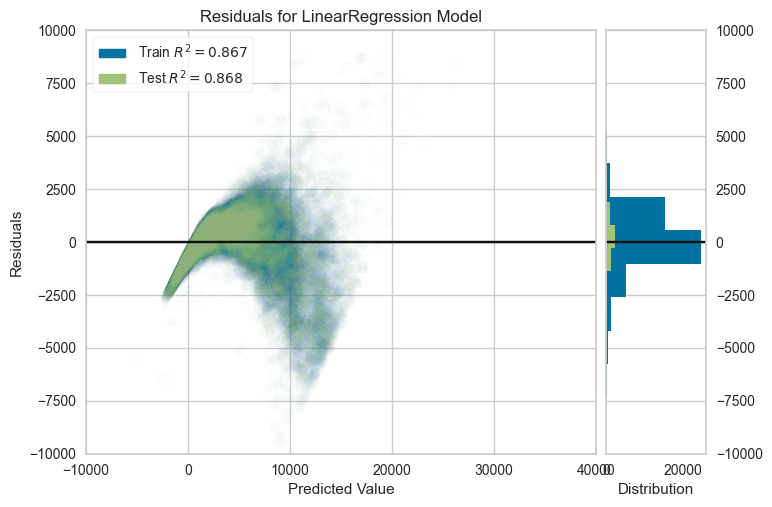
\includegraphics[width=\textwidth]{../Figures/question4/linresplot1.png}
        \caption[Network2]%
        {{Model \texttt{1} Residuals }}    
    \end{subfigure}
    \hfill
    \begin{subfigure}[b]{0.475\textwidth}  
        \centering 
        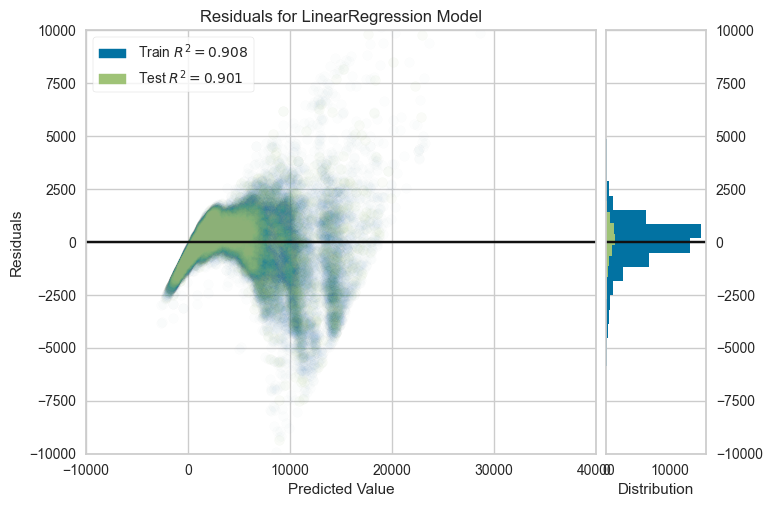
\includegraphics[width=\textwidth]{../Figures/question4/linresplot2.png}
        \caption[]%
        {Model \texttt{2} Residuals}    
    \end{subfigure}
    \vskip\baselineskip
    \begin{subfigure}[b]{0.475\textwidth}   
        \centering 
        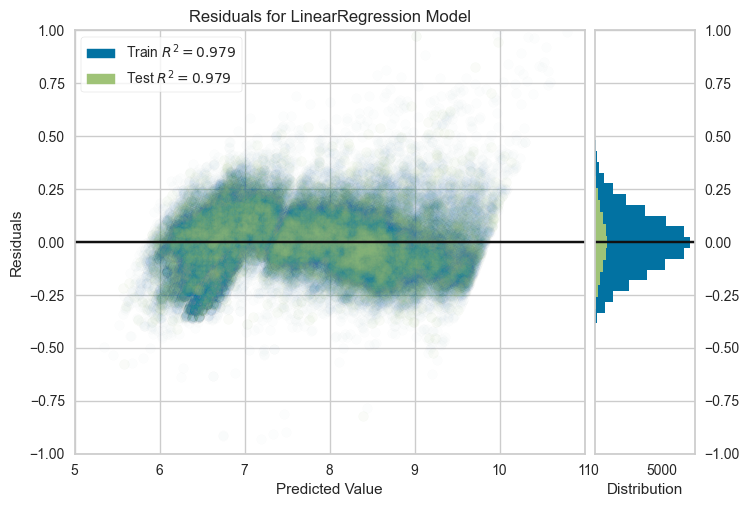
\includegraphics[width=\textwidth]{../Figures/question4/linresplot3.png}
        \caption[]%
        {{Model \texttt{3} $log$ Residual}}    
    \end{subfigure}
    \hfill
    \begin{subfigure}[b]{0.475\textwidth}   
        \centering 
        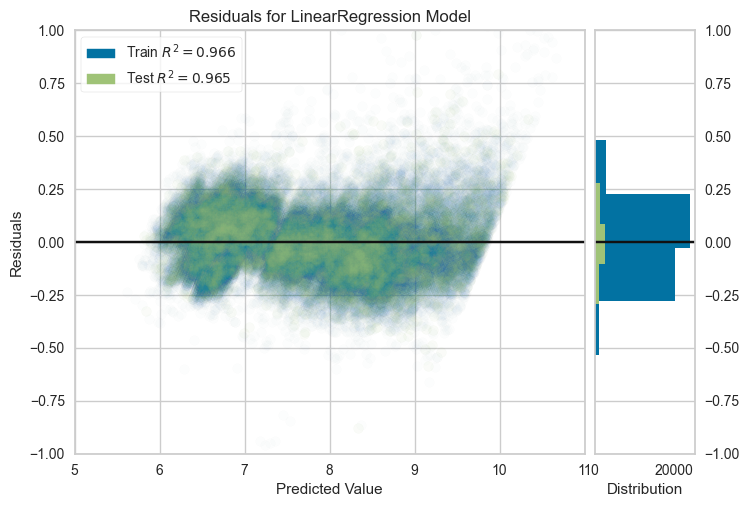
\includegraphics[width=\textwidth]{../Figures/question4/linresplot4.png}
        \caption[]%
        {{Model \texttt{4} $log$ Residuals}}    
    \end{subfigure}
    \caption{Residual Plots} 
\end{figure}
We then tested the linear regression model with processed data (deskewed as in 
Question 1.2) and unprocessed data. We noted that the model without processed features
seemed to perform much better as shown in Table 4 and visualized in Figure 5. Note that
Model \texttt{2}'s residual histogram is distributed far more sysmtetrically than 
Model \texttt{1}, implying that the linear regression fit better in this case.
However, we see in both Figures 5(a) and 5(b) that Models \texttt{1} and \texttt{2} 
predict many of the prices to be negative. \\\\
As such, we decided to test the model by taking the natural logrithm of 
\texttt{price} before fitting the regression. Note in Table 4 that with unprocessed 
Features, this model performed about the same, but with processed features the RSME 
decreased very significantly. We also see that our new $log$ residual plots seem to 
follow a linear trend, which makes sense as this implies that the error is increasing
as the price of the diamond itself increases. We also note that unlike earlier, Model
\texttt{3} has normally distributed residuals while Model \texttt{4} does not. This is
interesting, because this is the opposite of Models \texttt{1} and \texttt{2}; that is,
this time, the model with deskewed data has the more normal distribution of residuals.\\\\

Next, we test the Lasso Model by iterating through alpha values $10^k$ such that 
$k\in \mathbb{Z}$ and $-4 \geq k \leq 1$. We also try both the $log$(\texttt{price})
model, and try both with and without deskewing. \\\\

Next we test the Ridge model with all the same parameters are the Lasso model, except
we also test whether or not the 





\subsubsection*{Question 4.3}
\subsubsection*{Question 4.4}

\subsection*{Polynomial Regression}

\subsection*{Neural Network}

\subsection*{Random Forest}

\subsection*{LightGBM, CatBoost, and Bayesian Optimization}
\pagebreak
\begin{center}
    \begin{minipage}{10cm}
    	\begin{center}
    	\textbf{\large Project 4 Twitter Data}\\[0.1cm]
        \textbf{Inesh Chakrabarti, Lawrence Liu, Nathan Wei}\\[0.1cm]
    	\end{center}
    \end{minipage}\hfill
\end{center}
\rule{17cm}{0.1mm}



%%%%%%%%%%%%%%%%%%%%%%%%%%%%%%%%%%%%%%%%%%%%%%%%%%%%%%%%%%%%%%%%%%%%%%%%%%%%%%%%
%%%%%%%%%%%%%%%%%%%%%%%%%%%%%%%%%%%%%%%%%%%%%%%%%%%%%%%%%%%%%%%%%%%%%%%%%%%%%%%%




\end{document}

